% Options for packages loaded elsewhere
\PassOptionsToPackage{unicode}{hyperref}
\PassOptionsToPackage{hyphens}{url}
%
\documentclass[
]{article}
\usepackage{amsmath,amssymb}
\usepackage{iftex}
\ifPDFTeX
  \usepackage[T1]{fontenc}
  \usepackage[utf8]{inputenc}
  \usepackage{textcomp} % provide euro and other symbols
\else % if luatex or xetex
  \usepackage{unicode-math} % this also loads fontspec
  \defaultfontfeatures{Scale=MatchLowercase}
  \defaultfontfeatures[\rmfamily]{Ligatures=TeX,Scale=1}
\fi
\usepackage{lmodern}
\ifPDFTeX\else
  % xetex/luatex font selection
\fi
% Use upquote if available, for straight quotes in verbatim environments
\IfFileExists{upquote.sty}{\usepackage{upquote}}{}
\IfFileExists{microtype.sty}{% use microtype if available
  \usepackage[]{microtype}
  \UseMicrotypeSet[protrusion]{basicmath} % disable protrusion for tt fonts
}{}
\makeatletter
\@ifundefined{KOMAClassName}{% if non-KOMA class
  \IfFileExists{parskip.sty}{%
    \usepackage{parskip}
  }{% else
    \setlength{\parindent}{0pt}
    \setlength{\parskip}{6pt plus 2pt minus 1pt}}
}{% if KOMA class
  \KOMAoptions{parskip=half}}
\makeatother
\usepackage{xcolor}
\usepackage[margin=1in]{geometry}
\usepackage{color}
\usepackage{fancyvrb}
\newcommand{\VerbBar}{|}
\newcommand{\VERB}{\Verb[commandchars=\\\{\}]}
\DefineVerbatimEnvironment{Highlighting}{Verbatim}{commandchars=\\\{\}}
% Add ',fontsize=\small' for more characters per line
\usepackage{framed}
\definecolor{shadecolor}{RGB}{248,248,248}
\newenvironment{Shaded}{\begin{snugshade}}{\end{snugshade}}
\newcommand{\AlertTok}[1]{\textcolor[rgb]{0.94,0.16,0.16}{#1}}
\newcommand{\AnnotationTok}[1]{\textcolor[rgb]{0.56,0.35,0.01}{\textbf{\textit{#1}}}}
\newcommand{\AttributeTok}[1]{\textcolor[rgb]{0.13,0.29,0.53}{#1}}
\newcommand{\BaseNTok}[1]{\textcolor[rgb]{0.00,0.00,0.81}{#1}}
\newcommand{\BuiltInTok}[1]{#1}
\newcommand{\CharTok}[1]{\textcolor[rgb]{0.31,0.60,0.02}{#1}}
\newcommand{\CommentTok}[1]{\textcolor[rgb]{0.56,0.35,0.01}{\textit{#1}}}
\newcommand{\CommentVarTok}[1]{\textcolor[rgb]{0.56,0.35,0.01}{\textbf{\textit{#1}}}}
\newcommand{\ConstantTok}[1]{\textcolor[rgb]{0.56,0.35,0.01}{#1}}
\newcommand{\ControlFlowTok}[1]{\textcolor[rgb]{0.13,0.29,0.53}{\textbf{#1}}}
\newcommand{\DataTypeTok}[1]{\textcolor[rgb]{0.13,0.29,0.53}{#1}}
\newcommand{\DecValTok}[1]{\textcolor[rgb]{0.00,0.00,0.81}{#1}}
\newcommand{\DocumentationTok}[1]{\textcolor[rgb]{0.56,0.35,0.01}{\textbf{\textit{#1}}}}
\newcommand{\ErrorTok}[1]{\textcolor[rgb]{0.64,0.00,0.00}{\textbf{#1}}}
\newcommand{\ExtensionTok}[1]{#1}
\newcommand{\FloatTok}[1]{\textcolor[rgb]{0.00,0.00,0.81}{#1}}
\newcommand{\FunctionTok}[1]{\textcolor[rgb]{0.13,0.29,0.53}{\textbf{#1}}}
\newcommand{\ImportTok}[1]{#1}
\newcommand{\InformationTok}[1]{\textcolor[rgb]{0.56,0.35,0.01}{\textbf{\textit{#1}}}}
\newcommand{\KeywordTok}[1]{\textcolor[rgb]{0.13,0.29,0.53}{\textbf{#1}}}
\newcommand{\NormalTok}[1]{#1}
\newcommand{\OperatorTok}[1]{\textcolor[rgb]{0.81,0.36,0.00}{\textbf{#1}}}
\newcommand{\OtherTok}[1]{\textcolor[rgb]{0.56,0.35,0.01}{#1}}
\newcommand{\PreprocessorTok}[1]{\textcolor[rgb]{0.56,0.35,0.01}{\textit{#1}}}
\newcommand{\RegionMarkerTok}[1]{#1}
\newcommand{\SpecialCharTok}[1]{\textcolor[rgb]{0.81,0.36,0.00}{\textbf{#1}}}
\newcommand{\SpecialStringTok}[1]{\textcolor[rgb]{0.31,0.60,0.02}{#1}}
\newcommand{\StringTok}[1]{\textcolor[rgb]{0.31,0.60,0.02}{#1}}
\newcommand{\VariableTok}[1]{\textcolor[rgb]{0.00,0.00,0.00}{#1}}
\newcommand{\VerbatimStringTok}[1]{\textcolor[rgb]{0.31,0.60,0.02}{#1}}
\newcommand{\WarningTok}[1]{\textcolor[rgb]{0.56,0.35,0.01}{\textbf{\textit{#1}}}}
\usepackage{graphicx}
\makeatletter
\newsavebox\pandoc@box
\newcommand*\pandocbounded[1]{% scales image to fit in text height/width
  \sbox\pandoc@box{#1}%
  \Gscale@div\@tempa{\textheight}{\dimexpr\ht\pandoc@box+\dp\pandoc@box\relax}%
  \Gscale@div\@tempb{\linewidth}{\wd\pandoc@box}%
  \ifdim\@tempb\p@<\@tempa\p@\let\@tempa\@tempb\fi% select the smaller of both
  \ifdim\@tempa\p@<\p@\scalebox{\@tempa}{\usebox\pandoc@box}%
  \else\usebox{\pandoc@box}%
  \fi%
}
% Set default figure placement to htbp
\def\fps@figure{htbp}
\makeatother
\setlength{\emergencystretch}{3em} % prevent overfull lines
\providecommand{\tightlist}{%
  \setlength{\itemsep}{0pt}\setlength{\parskip}{0pt}}
\setcounter{secnumdepth}{-\maxdimen} % remove section numbering
\usepackage{bookmark}
\IfFileExists{xurl.sty}{\usepackage{xurl}}{} % add URL line breaks if available
\urlstyle{same}
\hypersetup{
  pdftitle={Soil Status (first project)},
  pdfauthor={Durjoy Kumar Sarker},
  hidelinks,
  pdfcreator={LaTeX via pandoc}}

\title{Soil Status (first project)}
\author{Durjoy Kumar Sarker}
\date{2025-10-05}

\begin{document}
\maketitle

\section{this is headline one}\label{this-is-headline-one}

\subsection{this is headline two}\label{this-is-headline-two}

\subsubsection{this is headline three}\label{this-is-headline-three}

\subsubsection{now I will create the bullet
list}\label{now-i-will-create-the-bullet-list}

\begin{itemize}
\tightlist
\item
  fist one is the sandy soil
\item
  2nd one is the clay soil
\item
  3rd one is loamy soil
\end{itemize}

\subsubsection{now create an numbered
list}\label{now-create-an-numbered-list}

\begin{enumerate}
\def\labelenumi{\arabic{enumi}.}
\tightlist
\item
  hi
\item
  hello
\item
  hallo
\end{enumerate}

\subsubsection{this is for the bold and
italic}\label{this-is-for-the-bold-and-italic}

\begin{itemize}
\tightlist
\item
  \textbf{high bold}
\item
  \emph{italic}
\item
  \textbf{\emph{Italic with bold}}
\end{itemize}

\subsubsection{add blockquotes}\label{add-blockquotes}

\begin{quote}
this is the blockquotes.
\end{quote}

\subsubsection{inline equation}\label{inline-equation}

\begin{itemize}
\tightlist
\item
  fertilizer formula: \(N + P + K = Fertilizer\ Rate\)
\end{itemize}

\subsubsection{block equation}\label{block-equation}

\[
Y = a + bX
\]

\subsubsection{link}\label{link}

\href{https://youtube.com}{youtube}

\subsubsection{image}\label{image}

\begin{figure}
\centering
\pandocbounded{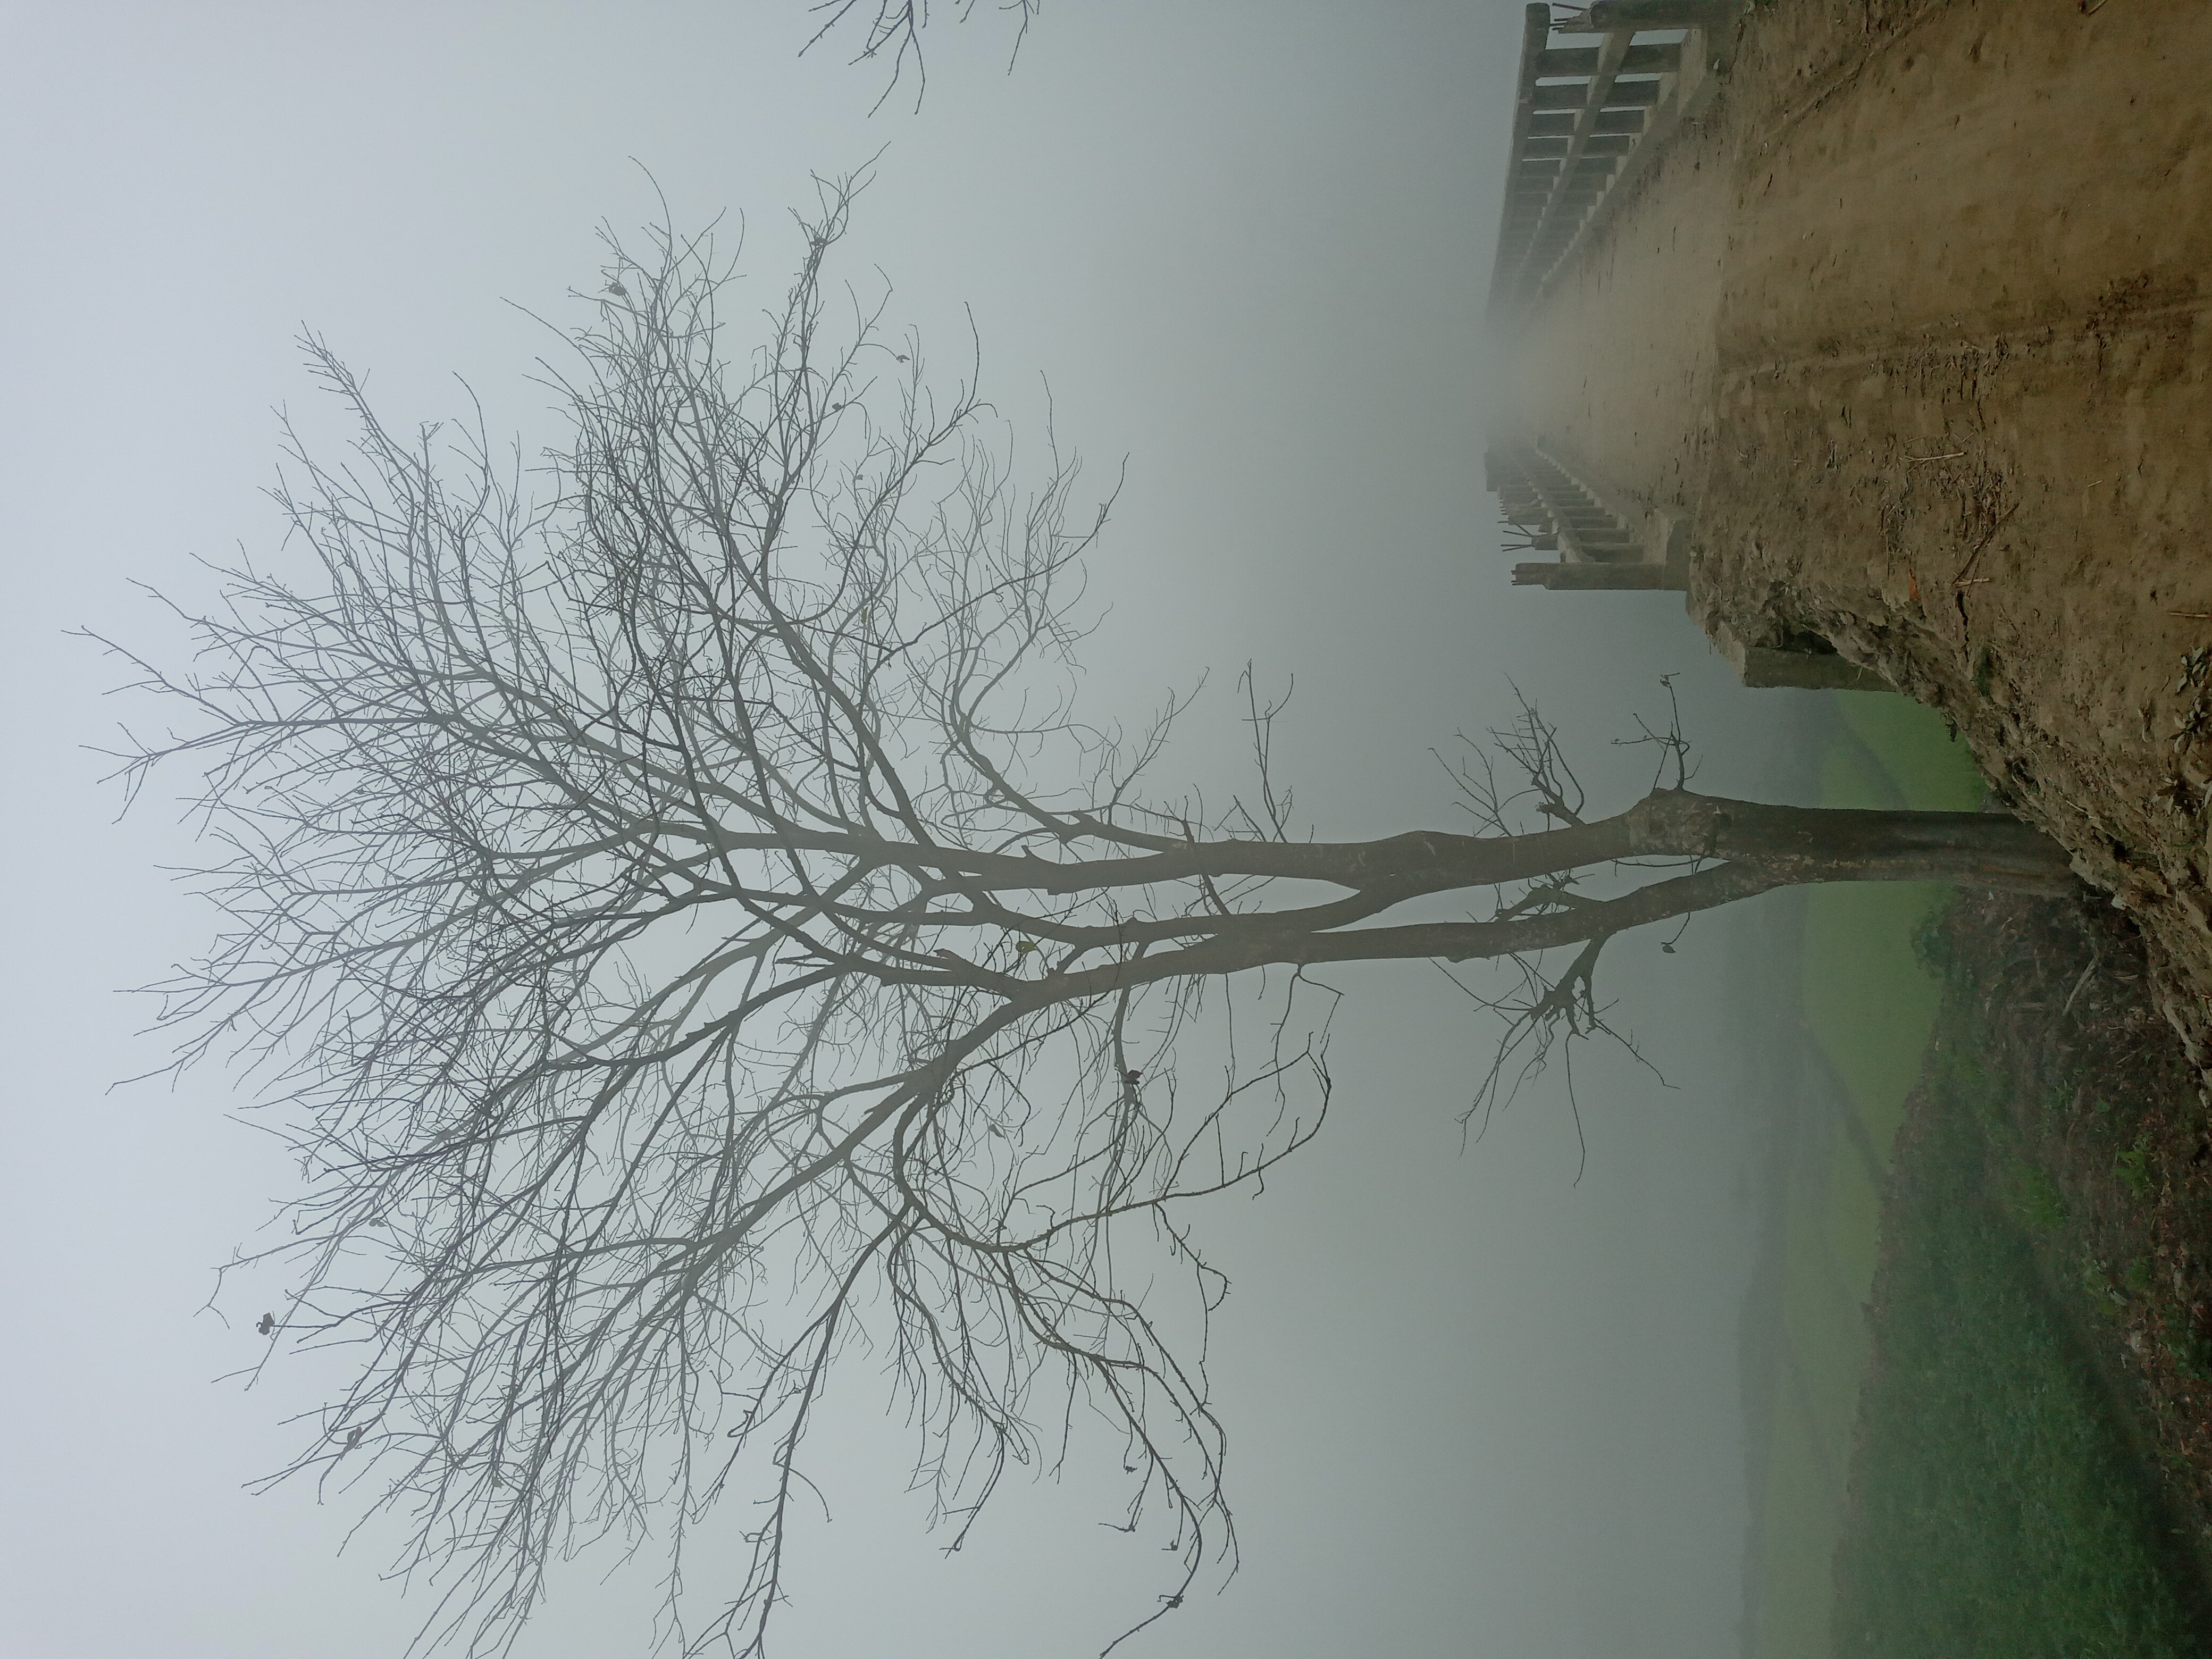
\includegraphics[keepaspectratio]{20210119_095246.jpg}}
\caption{figure:1}
\end{figure}

\subsubsection{inline code}\label{inline-code}

use \texttt{R} to analyze data

\section{Code Block}\label{code-block}

\begin{Shaded}
\begin{Highlighting}[]
\NormalTok{data }\OtherTok{=} \FunctionTok{read.csv}\NormalTok{(}\StringTok{"soil\_data.csv"}\NormalTok{)}
\FunctionTok{summary}\NormalTok{(data)}
\end{Highlighting}
\end{Shaded}

\begin{verbatim}
##  Soil_Sample              pH          Nitrogen    Phosphorus     Potassium 
##  Length:5           Min.   :5.80   Min.   :18   Min.   :12.0   Min.   :35  
##  Class :character   1st Qu.:5.90   1st Qu.:20   1st Qu.:14.0   1st Qu.:38  
##  Mode  :character   Median :6.20   Median :22   Median :15.0   Median :40  
##                     Mean   :6.28   Mean   :23   Mean   :15.4   Mean   :41  
##                     3rd Qu.:6.50   3rd Qu.:25   3rd Qu.:16.0   3rd Qu.:42  
##                     Max.   :7.00   Max.   :30   Max.   :20.0   Max.   :50  
##  Organic_Matter  Soil_Type        
##  Min.   :1.80   Length:5          
##  1st Qu.:1.90   Class :character  
##  Median :2.20   Mode  :character  
##  Mean   :2.28                     
##  3rd Qu.:2.50                     
##  Max.   :3.00
\end{verbatim}

\end{document}
